%beamer

% Comment/uncomment this line to toggle handout mode
\newcommand{\handout}{}

\ifdefined \handout
\documentclass[handout]{sdqbeamer} % Handout mode
\else
\documentclass{sdqbeamer}
\fi

%% UTF-8-Encoding
\usepackage[utf8]{inputenc}

% % \bigtimes abgeschrieben von http://tex.stackexchange.com/questions/14386/importing-a-single-symbol-from-a-different-font
% \DeclareFontFamily{U}{mathx}{\hyphenchar\font45}
% \DeclareFontShape{U}{mathx}{m}{n}{
%       <5> <6> <7> <8> <9> <10> gen * mathx
%       <10.95> mathx10 <12> <14.4> <17.28> <20.74> <24.88> mathx12
%       }{}
% \DeclareSymbolFont{mathx}{U}{mathx}{m}{n}
% \DeclareMathSymbol{\bigtimes}{\mathop}{mathx}{161}

\RequirePackage{xcolor}

\def\9{\square}
%\def\9{\blank}

% f"ur Aussagenlogik
\colorlet{alcolor}{blue}
\RequirePackage{tikz}
\usetikzlibrary{arrows.meta}
\newcommand{\alimpl}{\mathrel{\tikz[x={(0.1ex,0ex)},y={(0ex,0.1ex)},>={Classical TikZ Rightarrow[]}]{\draw[alcolor,->,line width=0.7pt,line cap=round] (0,0) -- (15,0);\path (0,-6);}}}
\newcommand{\alrimpl}{\mathrel{\tikz[x={(0.1ex,0ex)},y={(0ex,0.1ex)},>={Classical TikZ Leftarrow[]}]{\draw[alcolor,->,line width=0.7pt,line cap=round] (0,0) -- (15,0);\path (0,-6);}}}
\newcommand{\aleqv}{\mathrel{\tikz[x={(0.1ex,0ex)},y={(0ex,0.1ex)},>={Classical TikZ Rightarrow[]}]{\draw[alcolor,<->,line width=0.7pt,line cap=round] (0,0) -- (18,0);\path (0,-6);}}}
\newcommand{\aland}{\mathbin{\raisebox{-0.6pt}{\rotatebox{90}{\texttt{\color{alcolor}\char62}}}}}
\newcommand{\alor}{\mathbin{\raisebox{-0.8pt}{\rotatebox{90}{\texttt{\color{alcolor}\char60}}}}}
%\newcommand{\ali}[1]{_{\mathtt{\color{alcolor}#1}}}
\newcommand{\alv}[1]{\mathtt{\color{alcolor}#1}}
\newcommand{\alnot}{\mathop{\tikz[x={(0.1ex,0ex)},y={(0ex,0.1ex)}]{\draw[alcolor,line width=0.7pt,line cap=round,line join=round] (0,0) -- (10,0) -- (10,-4);\path (0,-8) ;}}}
\newcommand{\alvdash}{\mathrel{\tikz[x=4pt,y=3pt] {\draw[alcolor,line width=0.7pt,line cap=round,line join=round] (0,0) -- (0,1) -- (1,1) -- (0,1) -- (0,2);}}}
\newcommand{\alP}{\alv{P}} %ali{#1}}
\newcommand{\alQ}{\alv{Q}} %ali{#1}}
\newcommand{\alR}{\alv{R}} %ali{#1}}
\newcommand{\alS}{\alv{S}} %ali{#1}}
%\newcommand{\alka}{\negthinspace\hbox{\texttt{\color{alcolor}(}}}
\newcommand{\alka}{\negthinspace\text{\texttt{\color{alcolor}(}}}
%\newcommand{\alkz}{\texttt{\color{alcolor})}}\negthinspace}
\newcommand{\alkz}{\text{\texttt{\color{alcolor})}}\negthinspace}
\newcommand{\altrue}{\texttt{\textcolor{alcolor}{WAHR}}}
\newcommand{\alfalse}{\texttt{\textcolor{alcolor}{FALSCH}}}
\newcommand{\AAL}{A_{AL}}
\newcommand{\LAL}{\hbox{\textit{For}}_{AL}}
\newcommand{\AxAL}{\hbox{\textit{Ax}}_{AL}}
\newcommand{\AxEq}{\hbox{\textit{Ax}}_{Eq}}
\newcommand{\AxPL}{\hbox{\textit{Ax}}_{PL}}
\newcommand{\AALV}{\hbox{\textit{Var}}_{AL}}
\newcommand{\MP}{\hbox{\textit{MP}}}
\newcommand{\GEN}{\hbox{\textit{GEN}}}
\newcommand{\W}{\ensuremath{\hbox{\textbf{w}}}\xspace}
\newcommand{\F}{\ensuremath{\hbox{\textbf{f}}}\xspace}
\newcommand{\WF}{\ensuremath{\{\W,\F\}}\xspace}
\newcommand{\val}{\hbox{\textit{val}}}
\newcommand{\valDIb}{\val_{D,I,\beta}}

\newcommand*{\from}{\colon}

% die nachfolgenden Sachen angepasst an cmtt
\newlength{\ttquantwd}
\setlength{\ttquantwd}{1ex}
\newlength{\ttquantht}
\setlength{\ttquantht}{6.75pt}
\def\plall{%
  \tikz[line width=0.67pt,line cap=round,line join=round,baseline=(B),alcolor] {
    \draw (-0.5\ttquantwd,\ttquantht) -- node[coordinate,pos=0.4] (lll){} (-0.25pt,-0.0pt) -- (0.25pt,-0.0pt) -- node[coordinate,pos=0.6] (rrr){} (0.5\ttquantwd,\ttquantht);
    \draw (lll) -- (rrr);
    \coordinate (B) at (0,-0.35pt);
  }%
}
\def\plexist{%
  \tikz[line width=0.67pt,line cap=round,line join=round,baseline=(B),alcolor] {
    \draw (-0.9\ttquantwd,\ttquantht) -- (0,\ttquantht) -- node[coordinate,pos=0.5] (mmm){} (0,0) --  (-0.9\ttquantwd,0);
    \draw (mmm) -- ++(-0.75\ttquantwd,0);
    \coordinate (B) at (0,-0.35pt);
  }\ensuremath{\,}%
}
\let\plexists=\plexist
\newcommand{\NT}[1]{\ensuremath{\langle\mathrm{#1} \rangle}}

\newcommand{\CPL}{\text{\itshape Const}_{PL}}
\newcommand{\FPL}{\text{\itshape Fun}_{PL}}
\newcommand{\RPL}{\text{\itshape Rel}_{PL}}
\newcommand{\VPL}{\text{\itshape Var}_{PL}}
\newcommand{\ATer}{A_{\text{\itshape Ter}}}
\newcommand{\ARel}{A_{\text{\itshape Rel}}}
\newcommand{\AFor}{A_{\text{\itshape For}}}
\newcommand{\LTer}{L_{\text{\itshape Ter}}}
\newcommand{\LRel}{L_{\text{\itshape Rel}}}
\newcommand{\LFor}{L_{\text{\itshape For}}}
\newcommand{\NTer}{N_{\text{\itshape Ter}}}
\newcommand{\NRel}{N_{\text{\itshape Rel}}}
\newcommand{\NFor}{N_{\text{\itshape For}}}
\newcommand{\PTer}{P_{\text{\itshape Ter}}}
\newcommand{\PRel}{P_{\text{\itshape Rel}}}
\newcommand{\PFor}{P_{\text{\itshape For}}}

\newcommand{\plka}{\alka}
\newcommand{\plkz}{\alkz}
%\newcommand{\plka}{\plfoo{(}}
%\newcommand{\plkz}{\plfoo{)}}
\newcommand{\plcomma}{\hbox{\texttt{\color{alcolor},}}}
\newcommand{\pleq}{{\color{alcolor}\doteq}}

% MODIFIED (DJ)
% previously: \newcommand{\plfoo}[1]{\mathtt{\color{alcolor}#1}}
\newcommand{\plfoo}[1]{\texttt{\color{alcolor}#1}}

\newcommand{\plc}{\plfoo{c}}
\newcommand{\pld}{\plfoo{d}}
\newcommand{\plf}{\plfoo{f}}
\newcommand{\plg}{\plfoo{g}}
\newcommand{\plh}{\plfoo{h}}
\newcommand{\plx}{\plfoo{x}}
\newcommand{\ply}{\plfoo{y}}
\newcommand{\plz}{\plfoo{z}}
\newcommand{\plR}{\plfoo{R}}
\newcommand{\plS}{\plfoo{S}}

\newcommand{\bv}{\mathrm{bv}}
\newcommand{\fv}{\mathrm{fv}}

%\newcommand{\AxAL}{\hbox{\textit{Ax}}_{AL}}
%\newcommand{\AALV}{\hbox{\textit{Var}}_{AL}}

%\renewcommand{\#}[1]{\literal{#1}}
\newcommand{\A}{\mathcal{A}}
\newcommand{\Adr}{\text{Adr}}
\newcommand{\ar}{\mathrm{ar}}
\newcommand{\ascii}[1]{\literal{\char#1}}
%\newcommand{\assert}[1]{\text{/\!\!/\ } #1}
\newcommand{\assert}[1]{\colorbox{black!7!white}{\ensuremath{\{\;#1\;\}}}}
\newcommand{\Assert}[1]{$\langle$\textit{#1}$\rangle$}
\newcommand{\B}{\mathcal{B}}
\newcommand{\bfmod}{\mathbin{\kw{ mod }}}
\newcommand{\bb}{{\text{bb}}}
\def\bottom{\hbox{\small$\pmb{\bot}$}}
\newcommand{\card}[1]{|#1|}
%\newcommand{\cod}{\mathop{\text{cod}}}  % ist in thwmathabbrevs
\newcommand{\Conf}{\mathcal{C}}
\newcommand{\define}[1]{\emph{#1}}
%\renewcommand{\dh}{d.\,h.\@\xspace}
%\newcommand{\Dh}{D.\,h.\@\xspace}
%\newcommand{\engl}[1]{engl.\xspace\emph{#1}}
\newcommand{\eps}{\varepsilon}
%\newcommand{\evtl}{evtl.\@\xspace}
\newcommand{\fbin}{\text{bin}}
\newcommand{\finv}{\text{inv}}
\newcommand{\fnum}{\text{num}}
\newcommand{\fNum}{{\text{Num}}}
\newcommand{\frepr}{\text{repr}}
\newcommand{\fRepr}{\text{Repr}}
\newcommand{\fZkpl}{\text{Zkpl}}
\newcommand{\fLen}{\text{Len}}
\newcommand{\fsem}{\text{sem}}
\providecommand{\fspace}{\mathord{\text{space}}}
\providecommand{\fSpace}{\mathord{\text{Space}}}
\providecommand{\ftime}{\mathord{\text{time}}}
\providecommand{\fTime}{\mathord{\text{Time}}}
\newcommand{\fTrans}{\text{Trans}}
\newcommand{\fVal}{\text{Val}}

% MODIFIED (DJ)
\newcommand{\Val}{\text{Val}}

%\def\G{\mathbb{Z}}
\newcommand{\HT}[1]{\normalfont\textsc{HT-#1}}
\newcommand{\htr}[3]{\{#1\}\;#2\; \{#3\}}
\newcommand{\Id}{\text{I}}
%\newcommand{\ie}{i.\,e.\@\xspace}
\newcommand{\instr}[2]{\texttt{#1}\ \textit{#2}}
\newcommand{\Instr}[2]{\texttt{#1}\ \textrm{#2}}
\newcommand{\instrr}[3]{\texttt{#1}\ \textit{#2}\texttt{(#3)}}
\newcommand{\Instrr}[3]{\texttt{#1}\ \textrm{#2}\texttt{(#3)}}

% MODIFIED (DJ)
% previously:  \newcommand{\io}{\!\mid\!}
\newcommand{\io}{\ensuremath{\!\mid\!}}

%\usepackage{KITcolors}
\newcommand{\literal}[1]{\hbox{\textcolor{blue!95!white}{\textup{\texttt{\scalebox{1.11}{#1}}}}}}
%\newcommand{\literal}[1]{\hbox{\textcolor{KITblue!80!black}{\textup{\texttt{#1}}}}}
\def\kasten#1{\leavevmode\literal{\setlength{\fboxsep}{1pt}\fbox{\vrule  width 0pt height 1.5ex depth 0.5ex #1}}}
\newcommand{\kw}[1]{\ensuremath{\mathbf{#1}}}
\newcommand{\lang}[1]{\ensuremath{\langle#1\rangle}}
%\newcommand{\maw}{m.\,a.\,w.\@\xspace}
%\newcommand{\MaW}{M.\,a.\,w.\@\xspace}
\newcommand{\mdefine}[2][FOOBAR]{\define{#2}\def\foobar{FOOBAR}\def\optarg{#1}\ifx\foobar\optarg\def\optarg{#2}\fi\graffito{\optarg}}
\newcommand{\meins}{\rotatebox[origin=c]{180}{1}}
\newcommand{\Mem}{\text{Mem}}
\newcommand{\memread}{\text{memread}}
\newcommand{\memwrite}{\text{memwrite}}
\providecommand{\meta}[1]{\ensuremath{\langle}\textit{#1}\ensuremath{\rangle}}
%\newcommand{\N}{\mathbb{N}}
\newcommand{\NP}{\mathbf{NP}}
\newcommand{\Nadd}{N_{\text{add}}}
\newcommand{\Nmult}{N_{\text{mult}}}
% MODIFIED (DJ): added \!, mathcal{O}
\newcommand{\Oh}[1]{\mathcal{O}\!\left(#1\right)}
\newcommand{\Om}[1]{\Omega\!\left(#1\right)}
\newcommand{\personname}[1]{\textsc{#1}}
\newcommand{\regname}[1]{\texttt{#1}}
\newcommand{\mima}{\textsc{Mima}\xspace}
\newcommand{\mimax}{\textsc{Mima-X}\xspace}

\def\Pclass{\text{\bfseries P}}
\def\PSPACE{\text{\bfseries PSPACE}}

\newcommand{\SPush}{\text{push}}
\newcommand{\SPop}{\text{pop}}
\newcommand{\SPeek}{\text{peek}}
\newcommand{\STop}{\text{top}}
\newcommand{\STos}{\text{\itshape tos}}
\newcommand{\SBos}{\text{\itshape bos}}

%\newcommand{\R}{\mathbb{R}}
\newcommand{\Rnullplus}{\R_0^{+}}
\newcommand{\Rplus}{\R_{+}}
\newcommand{\resp}{resp.\@\xspace}
\newcommand{\Sem}{\text{Sem}}
\newcommand{\sgn}{\mathop{\text{sgn}}}
\newcommand{\sqbox}{\mathop{\raisebox{-6.2pt}{\hbox{\hbox to 0pt{$^{^{\sqcap}}$\hss}$^{^{\sqcup}}$}}}}
\newcommand{\sqleq}{\sqsubseteq}
\newcommand{\sqgeq}{\sqsupseteq}
% MODIFIED (DJ): added \!
\newcommand{\Th}[1]{\Theta\!\left(#1\right)}
%\newcommand{\usw}{usw.\@\xspace}
\newcommand{\V}[1]{\hbox{\textit{#1}}}
\newcommand{\x}{\times}
\newcommand{\ZK}{\mathbb{K}}
%\newcommand{\Z}{\mathbb{Z}}
\newcommand{\zB}{z.\,B.\@\xspace}
\newcommand{\ZB}{Z.\,B.\@\xspace}
% \newcommand{\bb}{{\text{bb}}}
% \def\##1{\hbox{\textcolor{darkblue}{\texttt{#1}}}}
% \def\A{\mathcal{A}}
% \newcommand{\0}{\#0}
% \newcommand{\1}{\#1}
% \newcommand{\Obj}{\text{Obj}}
% \newcommand{\start}{\mathop{\text{start}}}
% \newcommand{\compactlist}{\addtolength{\itemsep}{-\parskip}}
% \newcommand{\fval}{\text{val}}
% \newcommand{\lang}[1]{\ensuremath{\langle#1\rangle}}
% \newcommand{\io}{\!\mid\!}
% \def\sqbox{\mathop{\raisebox{-6.2pt}{\hbox{\hbox to 0pt{$^{^{\sqcap}}$\hss}$^{^{\sqcup}}$}}}}
% \def\sqleq{\sqsubseteq}
% \def\sqgeq{\sqsupseteq}
\def\Td{T_{\overline{d}}}
% \newcommand{\csym}[1]{\ensuremath{\#{c}_{\#{\hbox{\scriptsize #1}}}}}
% \newcommand{\F}{\ensuremath{\mathcal{F}}}
% \newcommand{\fsym}[2]{\ensuremath{\#{f}^{\#{\hbox{\scriptsize #1}}}_{\#{\hbox{\scriptsize #2}}}}}
% \newcommand{\rsym}[2]{\ensuremath{\#{R}^{\#{\hbox{\scriptsize #1}}}_{\#{\hbox{\scriptsize #2}}}}}
% \newcommand{\xsym}[1]{\ensuremath{\#{x}_{\#{\hbox{\scriptsize #1}}}}}
% \newcommand{\I}{\mathcal{I}}
% ********************************************************************
\usepackage{environ}
\usepackage{bm}
\usepackage{calc}
\usepackage{varwidth}
\usepackage{wasysym}
\usepackage{mathtools}


% Das ist der KIT-Stil
%\usepackage{../TutTexbib/beamerthemekit}
\titleimage{banner_2020_kit}
%\usetheme[deutsch,titlepage0]{KIT}

% Include PDFs
\usepackage{pdfpages}

% Libertine font (Original GBI font)
%\usepackage{libertine}
%\renewcommand*\familydefault{\sfdefault}  %% Only if the base font of the document is to be sans serif

% Nicer math symbols
\usepackage{eulervm}
%\usepackage{mathpazo}
\renewcommand\ttdefault{cmtt} % Computer Modern typewriter font, see lecture slides.

\usepackage{csquotes}

%%%%%%

%% Schönere Schriften
\usepackage[TS1,T1]{fontenc}

%% Bibliothek für Graphiken
\usepackage{graphicx}

%% der wird sowieso in jeder Datei gesetzt
\graphicspath{{../figures/}}

%% Anzeigetiefe für Inhaltsverzeichnis: 1 Stufe
\setcounter{tocdepth}{1}

%% Hyperlinks
\usepackage{hyperref}
% I don't know why, but this works and only includes sections and NOT subsections in the pdf-bookmarks.
\hypersetup{bookmarksdepth=subsection} 

%\usepackage{lmodern}
\usepackage{colortbl}
\usepackage[absolute,overlay]{textpos}
\usepackage{listings}
\usepackage{forloop}
%\usepackage{algorithmic} % PseudoCode package 

\usepackage{tikz}
\usetikzlibrary{matrix}
\usetikzlibrary{arrows.meta}
\usetikzlibrary{automata}
\usetikzlibrary{tikzmark}
\usetikzlibrary{positioning}

% Why has no-one come up with this yet? I mean, seriously. -.-
\tikzstyle{loop below right} = [loop, out=-60,in=-30, looseness=7]
\tikzstyle{loop below left} = [loop, out=-150,in=-120, looseness=7]
\tikzstyle{loop above right} = [loop, out=60,in=30, looseness=7]
\tikzstyle{loop above left} = [loop, out=150,in=120, looseness=7]
\tikzstyle{loop right below} = [loop below right]
\tikzstyle{loop left below} = [loop below left]
\tikzstyle{loop right above} = [loop above right]
\tikzstyle{loop left above} = [loop above left]

% Needed for gbi-macros
\usepackage{xspace}

%%%%%%

%% Verbatim
\usepackage{moreverb}

%%%%%%%%%%%%%%%%%%%%%%%%%%%%%%%%%%%% Copy end

%% Tabellen
\usepackage{array}
\usepackage{multicol}
\usepackage{hhline}

%% Bibliotheken für viele mathematische Symbole
\usepackage{amsmath, amsfonts, amssymb}

%% Deutsche Silbentrennung und Beschriftungen
\usepackage[ngerman]{babel}

%\usepackage{kbordermatrix}

% kbordermatrix settings
%\renewcommand{\kbldelim}{(} % Left delimiter
%\renewcommand{\kbrdelim}{)} % Right delimiter


% This is a configuration file with personal tutor information.
% It is therefore excluded from the git repository, so changes in this file will not conflict in git commits.

% Copy this template, rename to config.tex and add your information below.

\newcommand{\myname}{Lennart Rak}
\newcommand{\mymail}{lennart.rak@student.kit.edu} % Consider using your named student mail address to keep your u**** account private.
\newcommand{\mytutnumber}{02}

% Don't forget to update ILIAS url. WARNING: Underscores '_' and Ampersands '&' have to be escaped with backslashes '\'. Blame TeX, not me.
\newcommand{\myILIASurl}{http://s.kit.edu/gbi}

% Uncommenting this will print Socrative info with here defined roomname whenever \Socrative is called.
% (Otherwise, \Socrative will remain silent.)
% \newcommand{\mysocrativeroom}{???}

%\def\ThassesTut{}
\def\DanielsTut{}

\newcommand{\aboutMeFrame}{
	\begin{frame}{Über mich}
		\myname \\
		Informatik, 5. Fachsemester (Bachelor)
		
		% Lebensgeschichte...
		% Stammbaum...
		% Aufarbeitung der eigenen Todesser-Vergangenheit...
	\end{frame}
}
\newcommand{\aboutYouFrame}{
	\begin{frame}{Über euch}
	Wie heißt ihr? \\
	In welcher O-Phasen Gruppe wart ihr und was war euer Highlight? \\
	Habt ihr schon einen Partner zum Übungsblatt abgeben?
	    
	\end{frame}
}

\def\thisyear{2022}

% Update date of exam
\def\myKlausurtermin{27.~Februar~2023, 11:00–13:00~Uhr}

\def\mydate#1{
		  \ifnum#1=1\relax	  31. Oktober \thisyear \
	\else \ifnum#1=2\relax	  07. November \thisyear \
	\else \ifnum#1=3\relax    14. November \thisyear \
	\else \ifnum#1=4\relax    21. November \thisyear \
	\else \ifnum#1=5\relax    28. November \thisyear \
	\else \ifnum#1=6\relax    05. Dezember \thisyear \
	\else \ifnum#1=7\relax    12. Dezember \thisyear \
	\else \ifnum#1=8\relax    19. Dezember \thisyear \
	\else \ifnum#1=9\relax    09. Januar \thisyear \
	\else \ifnum#1=10\relax   16. Januar \nextyear \
	\else \ifnum#1=11\relax   23. Januar \nextyear \
	\else \ifnum#1=12\relax   30. Januar \nextyear \
	\else \ifnum#1=13\relax   06. Februar \nextyear \
	\else \ifnum#1=14\relax   13. Februar \nextyear \
	\else \textbf{Datum undefiniert!} 
	\fi\fi\fi\fi\fi\fi\fi\fi\fi\fi\fi\fi\fi\fi
}
\def\myshortdate#1{
		  \ifnum#1=1\relax	  31. 10 \thisyear \
	\else \ifnum#1=2\relax	  07. 11 \thisyear \
	\else \ifnum#1=3\relax    14. 11 \thisyear \
	\else \ifnum#1=4\relax    21. 11 \thisyear \
	\else \ifnum#1=5\relax    28. 11 \thisyear \
	\else \ifnum#1=6\relax    05. 12 \thisyear \
	\else \ifnum#1=7\relax    12. 12 \thisyear \
	\else \ifnum#1=8\relax    19. 12 \thisyear \
	\else \ifnum#1=9\relax    09. 01 \thisyear \
	\else \ifnum#1=10\relax   16. 01 \nextyear \
	\else \ifnum#1=11\relax   23. 01 \nextyear \
	\else \ifnum#1=12\relax   30. 01 \nextyear \
	\else \ifnum#1=13\relax   06. 02 \nextyear \
	\else \ifnum#1=14\relax   13. 02 \nextyear \
	\else \textbf{Datum undefiniert!} 
	\fi\fi\fi\fi\fi\fi\fi\fi\fi\fi\fi\fi\fi\fi
}

\def\mylasttimestext{Was bisher geschah...}

\colorlet{beamerlightred}{red!40}
\colorlet{beamerlightgreen}{green!50}
\colorlet{beamerlightyellow}{yellow!50}
\colorlet{lightred}{red!30}
\colorlet{lightgreen}{green!40}
\colorlet{lightyellow}{yellow!50}
\colorlet{fullred}{red!60}
\colorlet{fullgreen}{green}

\definecolor{myalertcolor}{rgb}{1,0.33,0.24}
\setbeamercolor{alerted text}{fg=myalertcolor}

% Flag to toggle display of KIT Logo.
% If you want to conform to the official logo guidelines, 
% you are not allowed to use the logo and should disable it
% using the following flag. Just saying.
% (But it's too beautiful, so best leave this commented. :P)
\newcommand{\noKITLogo}{}

% Toggle handout mode by including the following line before including PraeambelTut
% and removing the % at the start (but do NOT remove the % char here, otherwise handout mode will always be on!)
% Please keep handout mode off in all commits!

% \newcommand{\handout}{}



% define custom \handout command flag if handout mode is toggled  #DirtyAsHellButWell...
\only<beamer:0>{\def\handout{}} %beamer:0 == handout mode

\newcommand{\R}{\mathbb{R}}
\newcommand{\N}{\mathbb{N}}
\newcommand{\Z}{\mathbb{Z}}
\newcommand{\Q}{\mathbb{Q}}
\newcommand{\BB}{\mathbb{B}}
\newcommand{\C}{\mathbb{C}}
\newcommand{\K}{\mathbb{K}}
\newcommand{\G}{\mathbb{G}}
\newcommand{\nullel}{\mathcal{O}}
\newcommand{\einsel}{\mathds{1}}
\newcommand{\Pot}{\mathcal{P}}
\renewcommand{\O}{\text{O}}

\def\word#1{\hbox{\textcolor{blue}{\texttt{#1}}}}
\let\literal\word
\def\mword#1{\hbox{\textcolor{blue}{$\mathtt{#1}$}}}  % math word
\def\sp{\scalebox{1}[.5]{\textvisiblespace}}
\def\wordsp{\word{\sp}}

%\newcommand{\literal}[1]{\textcolor{blue}{\texttt{#1}}}
\newcommand{\realTilde}{\textasciitilde \ }
\newcommand{\setsize}[1]{\ensuremath{\left\lvert #1 \right\rvert}}
\newcommand{\size}[1]{\setsize{#1}}  % Shame on you, TeXStudio...
\newcommand{\set}[1]{\left\{#1\right\}}
\newcommand{\tuple}[1]{\left(#1\right)}
\newcommand{\normalvar}[1]{\text{$#1$}}

% Modified by DJ
\let\oldemptyset\emptyset
\let\emptyset\varnothing % proper emptyset

\newcommand{\boder}{\ensuremath{\mathbin{\textcolor{blue}{\vee}}}\xspace}
\newcommand{\bund}{\ensuremath{\mathbin{\textcolor{blue}{\wedge}}}\xspace}
\newcommand{\bimp}{\ensuremath{\mathrel{\textcolor{blue}{\to}}}\xspace}
\newcommand{\bgdw}{\ensuremath{\mathrel{\textcolor{blue}{\leftrightarrow}}}\xspace}
\newcommand{\bnot}{\ensuremath{\textcolor{blue}{\neg}}\xspace}
\newcommand{\bone}{\ensuremath{\textcolor{blue}{1}}\text{}}
\newcommand{\bzero}{\ensuremath{\textcolor{blue}{0}}\text{}}
\newcommand{\bleftBr}{\ensuremath{\textcolor{blue}{\texttt{(}}}\text{}}
\newcommand{\brightBr}{\ensuremath{\textcolor{blue}{\texttt{)}}}\text{}}

% Fix of \b... commands:

\renewcommand{\boder}{\alor}
\renewcommand{\bund}{\aland}
\renewcommand{\bimp}{\alimpl}
\renewcommand{\bgdw}{\aleqv}
\renewcommand{\bnot}{\alnot}
\renewcommand{\bleftBr}{\alka}
\renewcommand{\brightBr}{\alkz}
\newcommand{\alA}{\word A}
\newcommand{\alB}{\word B}
\newcommand{\alC}{\word C}

\newcommand{\plB}{\plfoo{B}}
\newcommand{\plE}{\plfoo{E}}

\newcommand{\summe}[2]{\sum\limits_{#1}^{#2}}
\newcommand{\limes}[1]{\lim\limits_{#1}}

%\newcommand{\numpp}{\advance \value{weeknum} by -2 \theweeknum \advance \value{weeknum} by 2}
%\newcommand{\nump}{\advance \value{weeknum} by -1 \theweeknum \advance \value{weeknum} by 1}

\newcommand{\mycomment}[1]{}
\newcommand{\Comment}[1]{}

%% DISCLAIMER START 
% It is INSANELY IMPORTANT NOT TO DO THIS OUTSIDE BEAMER CLASS! IN ARTCILE DOCUMENTS, THIS IS VERY LIKELY TO BUG AROUND!
\makeatletter%
\@ifclassloaded{beamer}%
{
	% TODO 
	% no time... later.   (= never -.-)
	% redefine section to ignore multiple \section calls with the same title
}%
{
	\errmessage{ERROR: section command redefinition outside of beamer class document! Please contact the author of this code or read the F-ing disclaimer.}
}%
\makeatother%
%% DISCLAIMER END

\newcounter{abc}
\newenvironment{alist}{
  \begin{list}{(\alph{abc})}{
      \usecounter{abc}\setlength{\leftmargin}{8mm}\setlength{\labelsep}{2mm}
    }
}{\end{list}}


\newcommand{\stdarraystretch}{1.20}
\renewcommand{\arraystretch}{\stdarraystretch}  % for proper row spacing in tables

\newcommand{\morescalingdelimiters}{   % for proper \left( \right) typography
	\delimitershortfall=-1pt  
	\delimiterfactor=1
}

\newcommand{\centered}[1]{\vspace{-\baselineskip}\begin{center}#1\end{center}\vspace{-\baselineskip}}

% for \implitem and \item[bla] stuff to look right:
\setbeamercolor*{itemize item}{fg=black}
\setbeamercolor*{itemize subitem}{fg=black}
\setbeamercolor*{itemize subsubitem}{fg=black}

\setbeamercolor*{description item}{fg=black}
\setbeamercolor*{description subitem}{fg=black}
\setbeamercolor*{description subsubitem}{fg=black}

\renewcommand{\qedsymbol}{\textcolor{black}{\openbox}}

\renewcommand{\mod}{\mathop{\textbf{mod}}}
\renewcommand{\div}{\mathop{\textbf{div}}}

\newcommand{\ceil}[1]{\left\lceil#1\right\rceil}
\newcommand{\floor}[1]{\left\lfloor#1\right\rfloor}
\newcommand{\abs}[1]{\left\lvert #1 \right\rvert}
\newcommand{\Matrix}[1]{\begin{pmatrix} #1 \end{pmatrix}}
\newcommand{\braced}[1]{\left\lbrace #1 \right\rbrace}

% "something" placeholder. Useful for repairing spacing of operator sections, like `\sth = 42`.
\def\sth{\vphantom{.}}

\def\fract#1/#2 {\frac{#1}{#2}} % ! Trailing space is crucial!
\def\dfract#1/#2 {\dfrac{#1}{#2}} % ! Trailing space is crucial!

\newcommand{\Mid}{\;\middle|\;}

\let\after\circ



\def\·{\cdot}
\def\*{\cdot}
\def\?>{\ensuremath{\rightsquigarrow}}  % Fuck you, Latex
\def\~~>{\ensuremath{\rightsquigarrow}}  

\newcommand{\tight}[1]{{\renewcommand{\arraystretch}{0.76} #1}}
\newcommand{\stackedtight}[1]{\renewcommand{\arraystretch}{0.76} \begin{matrix} #1 \end{matrix} }
\newcommand{\stacked}[1]{\begin{matrix} #1 \end{matrix} }
\newcommand{\casesl}[1]{\delimitershortfall=0pt  \left\lbrace\hspace{-.3\baselineskip}\begin{array}{ll} #1 \end{array}\right.}
\newcommand{\casesr}[1]{\delimitershortfall=0pt  \left.\begin{array}{ll} #1 \end{array}\hspace{-.3\baselineskip}\right\rbrace}
\newcommand{\caseslr}[1]{\delimitershortfall=0pt  \left\lbrace\hspace{-.3\baselineskip}\begin{array}{ll} #1 \end{array}\hspace{-.3\baselineskip}\right\rbrace}

\def\q#1uad{\ifnum#1=0\relax\else\quad\q{\the\numexpr#1-1\relax}uad\fi}
% e.g. \q1uad = \quad, \q2uad = \qquad etc.

\newcommand{\qqquad}{\q3uad}
\newcommand{\minusquad}{\hspace{-1em}}

%% Placeholder utils
% \§{#1}   Saves #1 as placeholder and prints it
% \.       Prints an \hphantom with the size of the recalled placeholder.
\def\indentstring{}
\def\§#1{\def\indentstring{#1}#1}
\def\.{{$\hphantom{\text{\indentstring}}$}}
%% Placeholder utils end

\newcommand{\impl}{\ifmmode\ensuremath{\mskip\thinmuskip\Rightarrow\mskip\thinmuskip}\else$\Rightarrow$\fi\xspace}
\newcommand{\Impl}{\ifmmode\implies\else$\Longrightarrow$\fi\xspace}

\newcommand{\derives}{\Rightarrow}

\newcommand{\gdw}{\ifmmode\mskip\thickmuskip\Leftrightarrow\mskip\thickmuskip\else$\Leftrightarrow$\fi\xspace}
\newcommand{\Gdw}{\ifmmode\iff\else$\Longleftrightarrow$\fi\xspace}

% Legacy code from the algo tutorial slides. Perhaps useful. Try with care.
\mycomment{
	\newcommand{\impl}{\ifmmode\ensuremath{\mskip\thinmuskip\Rightarrow\mskip\thinmuskip}\else$\Rightarrow$\xspace\fi}  
	\newcommand{\Impl}{\ifmmode\implies\else$\Longrightarrow$\xspace\fi}
	
	\newcommand{\gdw}{\ifmmode\mskip\thickmuskip\Leftrightarrow\mskip\thickmuskip\else$\Leftrightarrow$\xspace\fi}
	\newcommand{\Gdw}{\ifmmode\iff\else$\Longleftrightarrow$\xspace\fi}
}
	
\newcommand{\gdwdef}{\ifmmode\mskip\thickmuskip:\Leftrightarrow\mskip\thickmuskip\else:$\Leftrightarrow$\xspace\fi}
\newcommand{\Gdwdef}{\ifmmode\mskip\thickmuskip:\Longleftrightarrow\mskip\thickmuskip\else:$\Longleftrightarrow$\xspace\fi}

\newcommand{\symbitemnegoffset}{\hspace{-.5\baselineskip}}
\newcommand{\implitem}{\item[\impl\symbitemnegoffset]}
\newcommand{\Implitem}{\item[\Impl\symbitemnegoffset]}


\newcommand{\forcenewline}{\mbox{}\\}

\newcommand{\bfalert}[1]{\textbf{\alert{#1}}}
\let\elem\in   % I'm a Haskell freak. Don't judge me. :P


\def\|#1|{\text{\normalfont #1}}  % | steht für senkrecht (anstatt kursiv wie sonst im math mode)


% proper math typography
\newcommand{\functionto}{\longrightarrow}
\renewcommand{\geq}{\geqslant}
\renewcommand{\leq}{\leqslant}
\let\oldsubset\subset
\renewcommand{\subset}{\subseteq} % for all idiots out there using subset

\newenvironment{threealign}{%
	\[
	\begin{array}{r@{\ }c@{\ }l}
}{%
	\end{array}	
	\]
}

\newcommand{\concludes}{ \\ \hline  }
\newcommand{\deduction}[1]{
	\begin{varwidth}{.8\linewidth}
		\begin{tabular}{>{$}c<{$}}
			#1
		\end{tabular}
	\end{varwidth}	
}

\definecolor{hoareorange}{rgb}{1,.85,.6}
\newcommand{\hoareassert}[1]{\setlength{\fboxsep}{1pt}\setlength{\fboxrule}{-1.4pt}\fcolorbox{white}{hoareorange}{\ensuremath{\{\;#1\;\}}}\setlength\fboxrule{\defaultfboxrule}\setlength{\fboxsep}{3pt}}

\newcommand{\mailto}[1]{\href{mailto:#1}{{\textcolor{blue}{\underline{#1}}}}}
\newcommand{\urlnamed}[2]{\href{#2}{\textcolor{blue}{\underline{#1}}}}
\renewcommand{\url}[1]{\urlnamed{#1}{#1}}

\newcommand{\hanging}{\hangindent=0.7cm}
\newcommand{\indented}{\hanging}


% \hstretchto prints #2 left-aligned into a box of the width of #1
\def\hstretchto#1#2{%
	\mbox{}\vphantom{#2}\rlap{#2}\hphantom{#1}%
}

\def\vstretchto#1#2{%
	\mbox{}\hphantom{#2}\smash{#2}\vphantom{#1}%
}

% \hstretchtocentered prints #2 centered into a box of the width of #1
\def\hstretchtocentered#1#2{%
	\mbox{}\vphantom{#2}\scalebox{0.5}{\hphantom{#1}}\clap{#2}\scalebox{0.5}{\hphantom{#1}}%
}

% vertical centering
\newcommand{\vertcenter}[1]{%
	\ensuremath{\vcenter{\hbox{#1}}}%
}


%requires \thisyear to be defined (s. config.tex)!
\edef\nextyear{\the\numexpr\thisyear+1\relax}


% --- \frameheight constant ---
\newlength\fullframeheight
\newlength\framewithtitleheight
\setlength\fullframeheight{.92\textheight}
\setlength\framewithtitleheight{.86\textheight}

\newlength\frameheight
\setlength\frameheight{\fullframeheight}

\let\frametitleentry\relax
\let\oldframetitle\frametitle
\def\newframetitle#1{\global\def\frametitleentry{#1}\if\relax\frametitleentry\relax\else\setlength\frameheight{\framewithtitleheight}\fi\oldframetitle{#1}}
\let\frametitle\newframetitle

\def\newframetitleoff{\let\frametitle\oldframetitle}
\def\newframetitleon{\let\frametitle\newframetitle}
% --- \frameheight constant end ---

\newcommand{\fakeframetitle}[1]{%
	\vspace{-2.05\baselineskip}%
	{\Large \textbf{#1}} \\%
	\smallskip
}



\newenvironment{headframe}{\Huge THIS IS AN ERROR. PLEASE CONTACT THE ADMIN OF THIS TEX CODE. (headframe env def failed)}{}
\RenewEnviron{headframe}[1][]{
	\begin{frame}\frametitle{\ }
		\centering
		\Huge\textbf{\textsc{\BODY} \\
		}
		\Large {#1}
		\frametitle{\ }
	\end{frame}
}


\makeatletter
% Provides color if undefined.
\newcommand{\colorprovide}[2]{%
	\@ifundefinedcolor{#1}{\colorlet{#1}{#2}}{}}
\makeatother


\colorprovide{lightred}{red!30}
\colorprovide{lightgreen}{green!40}
\colorprovide{lightyellow}{yellow!50}
\colorprovide{lightblue}{blue!10}
\colorprovide{beamerlightred}{lightred}
\colorprovide{beamerlightgreen}{lightgreen}
\colorprovide{beamerlightyellow}{lightyellow}
\colorprovide{beamerlightblue}{lightblue}
\colorprovide{fullred}{red!60}
\colorprovide{fullgreen}{green}
\definecolor{darkred}{RGB}{115,48,38}
\definecolor{darkgreen}{RGB}{48,115,38}
\definecolor{darkyellow}{RGB}{100,100,0}

\only<handout:0>{\colorlet{adaptinglightred}{beamerlightred}}
\only<handout:0>{\colorlet{adaptinglightgreen}{beamerlightgreen}}
\only<handout:0>{\colorlet{adaptinglightyellow}{beamerlightyellow}}
\only<handout:0>{\colorlet{adaptinglightblue}{beamerlightblue}}
\only<beamer:0>{\colorlet{adaptinglightred}{lightred}}
\only<beamer:0>{\colorlet{adaptinglightgreen}{lightgreen}}
\only<beamer:0>{\colorlet{adaptinglightyellow}{lightyellow}}
\only<beamer:0>{\colorlet{adaptinglightblue}{lightblue}}
\only<handout:0>{\colorlet{adaptingred}{lightred}}
\only<beamer:0>{\colorlet{adaptingred}{fullred}}
\only<handout:0>{\colorlet{adaptinggreen}{lightgreen}}
\only<beamer:0>{\colorlet{adaptinggreen}{fullgreen}}



\newcommand{\TrueQuestion}[1]{
	\TrueQuestionE{#1}{}
}

\newcommand{\YesQuestion}[1]{
	\YesQuestionE{#1}{}
}

\newcommand{\FalseQuestion}[1]{
	\FalseQuestionE{#1}{}
}

\newcommand{\NoQuestion}[1]{
	\NoQuestionE{#1}{}
}

\newcommand{\DependsQuestion}[1]{
	\DependsQuestionE{#1}{}
}

\newcommand{\QuestionVspace}{\vspace{4pt}}
\newcommand{\QuestionParbox}[1]{\begin{varwidth}{.85\linewidth}#1\end{varwidth}}
\newcommand{\ExplanationParbox}[1]{\begin{varwidth}{.97\linewidth}#1\end{varwidth}}
\colorlet{questionlightgray}{gray!23}
\let\defaultfboxrule\fboxrule

% #1: bg color
% #2: fg color short answer
% #3: short answer text
% #4: question
% #5: explanation
\newcommand{\GenericQuestion}[5]{
	\setlength\fboxrule{2pt}
	\only<+|handout:0>{\hspace{-2pt}\fcolorbox{white}{questionlightgray}{\QuestionParbox{#4} \quad\textbf{?}}}
	\visible<+->{\hspace{-2pt}\fcolorbox{white}{#1}{\QuestionParbox{#4} \quad\textbf{\textcolor{#2}{#3}}} \if\relax#5\relax\else\ExplanationParbox{#5}\fi} \\
	\setlength\fboxrule{\defaultfboxrule}
}

% #1: Q text
% #2: Explanation
\newcommand{\TrueQuestionE}[2]{
	\GenericQuestion{adaptinglightgreen}{darkgreen}{Wahr.}{#1}{#2}
}

% #1: Q text
% #2: Explanation
\newcommand{\YesQuestionE}[2]{
	\GenericQuestion{adaptinglightgreen}{darkgreen}{Ja.}{#1}{#2}
}

% #1: Q text
% #2: Explanation
\newcommand{\FalseQuestionE}[2]{
	\GenericQuestion{adaptinglightred}{darkred}{Falsch.}{#1}{#2}
}

% #1: Q text
% #2: Explanation
\newcommand{\NoQuestionE}[2]{
	\GenericQuestion{adaptinglightred}{darkred}{Nein.}{#1}{#2}
}

% #1: Q text
% #2: Explanation
\newcommand{\DependsQuestionE}[2]{
	\GenericQuestion{adaptinglightyellow}{darkyellow}{Je nachdem!}{#1}{#2}
}

% #1: Q text
% #2: Answer
\newcommand{\ContentQuestion}[2]{
	\GenericQuestion{adaptinglightblue}{black}{\minusquad}{#1}{#2}
}

%\ifnum\thisyear=2018 \else \errmessage{Old ILIAS link inside preamble. Please update.} \fi

\newcommand{\ILIAS}{\urlnamed{ILIAS}{\myILIASurl}\xspace}
\newcommand{\Klausurtermin}{\myKlausurtermin\xspace}

\newcommand{\Socrative}{\ifdefined\mysocrativeroom \only<handout:0>{socrative.com $\quad \~~> \quad $ Student login \\ Raumname:  \mysocrativeroom\\ \medskip}\else\fi}

\newcommand{\thasse}[1]{
	\ifdefined\ThassesTut #1\xspace \else\fi
}
\newcommand{\daniel}[1]{
	\ifdefined\DanielsTut #1\xspace \else\fi
}
\newcommand{\thassedaniel}[2]{\ifdefined\ThassesTut #1\else\ifdefined\DanielsTut #2\fi\fi\xspace}

\ifdefined\ThassesTut \ifdefined\DanielsTut \errmessage{ERROR: Both ThassesTut and DanielsTut flags are set. This is most likely an error. Please check your config.tex file.} \else \fi \else \ifdefined\DanielsTut \else \errmessage{ERROR: Neither ThassesTut  nor DanielsTut flags are set. This is most likely an error. Please check your config.tex file.} \fi\fi

%\newcommand{\sgn}{\text{sgn}}

%%%%%%%%%%%% INHALT %%%%%%%%%%%%%%%%

%% Wochennummer
\newcounter{weeknum}

%% Titelinformationen
\title[GBI-Tutorium \mytutnumber, Woche \theweeknum]{Grundbegriffe der Informatik Tutorium \mytutnumber}

\subtitle{Woche \theweeknum \xspace}
\author[\myname]{\myname \xspace \normalfont (\mailto{\mymail})}
\groupname{KIT -- Karlsruher Institut für Technologie}
\date[\myshortdate{\theweeknum}]{\mydate{\theweeknum}}

% Modified, DJ (better safe than sorry)
%\AuthorTitleSep{ – }

%% Titel einfügen
\newcommand{\titleframe}{\KITtitleframe}

%% Alles starten mit \starttut{X}
\newcommand{\starttut}[1]{\setcounter{weeknum}{#1}\pdfinfo{
		/Author (\myname)
		/Title  (GBI-Tutorium \mytutnumber, Woche \theweeknum)
	}\titleframe\frame{\frametitle{Inhalt}\tableofcontents} \AtBeginSection[]{%
		\begin{frame}{Wo sind wir gerade?}
		\tableofcontents[currentsection]
	\end{frame}\addtocounter{framenumber}{-1}}}


\newcommand{\framePrevEpisode}{
\begin{headframe}
	\mylasttimestext
\end{headframe}
}

\newcommand{\lastframetitled}[6]{
% 	\frame{\frametitle{#6}
% 		\vspace{-#2\baselineskip}
% 		\begin{figure}[H]
% 			\centering
% 			\LARGE \textbf{\textsc{#5}} \\
% 			\vspace{.2\baselineskip}
% 			\includegraphics[#1]{#3}
% 			\vspace{-6pt}
% 			\begin{center}
% 				\small \url{#4} 
% 			\end{center}
% 		\end{figure} 
% 	}
\begin{frame}[plain]
    \vspace{\baselineskip}
    \centering
    \Large\textbf{#6}
    \begin{figure}[H]
		\centering
% 		\LARGE \textbf{\textsc{#5}} \\
% 		\vspace{.2\baselineskip}
		\includegraphics[#1]{#3}
		\vspace{-6pt}
		\begin{center}
			\small \url{#4} 
		\end{center}
	\end{figure}
\end{frame}
}

% #1 number
% #2 title 
% #3 vspace (positive) without unit (\baselineskip)
\newcommand{\xkcdframe}[3]{
	\lastframetitled{width=.96\textwidth}{#3}{xkcd/#1}{http://xkcd.com/#1}{}{#2}
}

\newcommand{\xkcdframevert}[3]
{
	\lastframetitled{height=.96\frameheight}{#3}{xkcd/#1}{http://xkcd.com/#1}{}{#2}
}

% #1 number
% #2 title 
% #3 vspace (positive) without unit (\baselineskip)
% #4 \includegraphics[] optional parameters
\newcommand{\xkcdframecustom}[4]
{
	\lastframetitled{#4}{#3}{xkcd/#1}{http://xkcd.com/#1}{}{#2}
}

\newcommand{\slideThanks}{
	\begin{frame}
	\frametitle{Credits}
	\begin{block}{}
		An der Erstellung des Foliensatzes haben mitgewirkt:\\[1em]
		Daniel Jungkind \\
		Thassilo Helmold \\
		Philipp Basler \\
		Nils Braun \\
		Dominik Doerner \\
		Ou Yue \\
	\end{block}
\end{frame}
}

%% Wörter DEPRECATED! DO NOT USE
\newcommand{\code}[1]{$\mathbf{#1}$}

\morescalingdelimiters

\begin{document}
\starttut{5}

\begin{frame}{Zu Blatt \#4}
	
	Schnitt: \quad 10 / 20~P
	
	\pause
	\begin{figure}
	    \centering
	    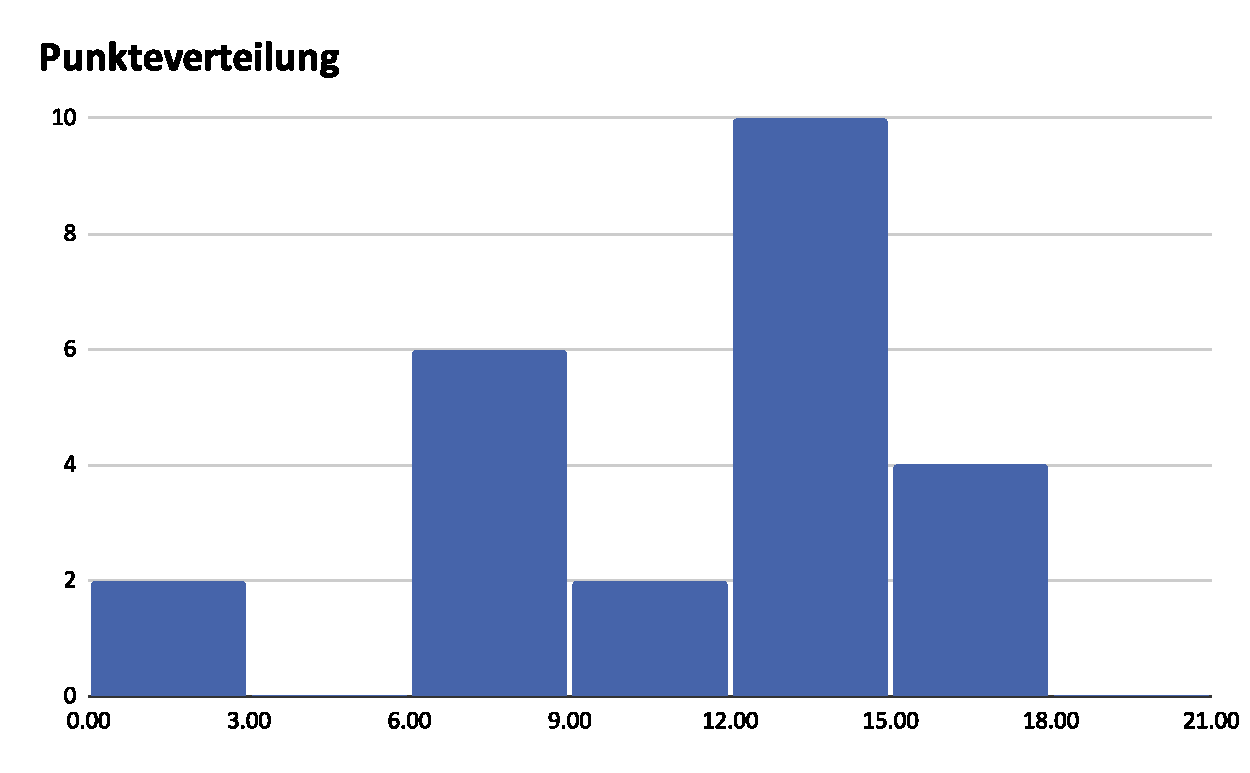
\includegraphics[scale=0.45]{./Punkteverteilung.pdf}
	\end{figure}
\end{frame}

% Zum Aufwärmen: PEBA Tutorenprogramm Aktivierung Code merken (PDF im gleichen Ordner zu finden)

 \framePrevEpisode


 
\begin{frame}{Rückblick}
	Auf formale Sprachen können wir \textbf{ähnliche} Operationen anwenden wie auf Wörtern:
	\begin{itemize}
		\item $L_1 \cdot L_2 = \{w_1 w_2 \mid w_1 \in L_1 \text{ und } w_2 \in L_2 \}$\\
		Jeweils ein Wort aus $L_1$ konkateniert mit einem Wort aus $L_2$.
		\pause
		\item $L^0 = \{\varepsilon \}, \qquad L^{i+1} = L^i \cdot L$\\
		Alle Wörter, die aus $i = 0,1,2...$ Wörtern der Sprache zusammengesetzt wurden
		\pause
		\item $L^+ = \bigcup \limits_{i=1}^\infty L^i \qquad L^* = L^+ \cup L^0$\\
		Alle Wörter, die sich aus den Wörtern der Sprache bilden lassen \\ 
		(ohne/mit zusätzlichem $\eps$ als Würze).
	\end{itemize}
	Ein Alphabet selbst ist \textbf{auch} ne formale Sprache, nämlich mit Wörtern der Länge 1.
\end{frame}

\begin{frame}[t]{Wahr oder falsch?}
	\FalseQuestionE{Jede Sprache enthält Wörter.}{ $\emptyset$ ist auch eine gültige Sprache.}
	\FalseQuestionE{$\word{0}^* = \{\eps, \word{0}, \word{00}, \word{000}, ...\}$}{$\word{0}^*$ gibt es nicht, denn $\word{0} \neq \{\word{0}\}$.}
	\TrueQuestionE{Es gibt Sprachen $L$, für die gilt $\eps \in L^+$.}{\ZB $L = \set{\eps, \word{aaa}}$.}
	\FalseQuestionE{$L^+ = L^* \setminus L^0$.}{Gilt nicht, wenn $\varepsilon \in L$.}
	\TrueQuestionE{$\{\}^* \neq \{\} $.}{ $\{\}^* = \{\varepsilon\}$.}	
\end{frame}

\section{Von der Darstellung zur Zahl}

\subsection{Definitionen}
\begin{frame}{Numerischer Wert einer Ziffernfolge}
	\begin{Definition}
		Zu einer Zahlenbasis $b$ definiere 
		\begin{align*}
			\fnum_b &\from Z_b \functionto \Z \\
			\fnum_b(x) &:= x \text{ (als Zahl)} \quad \text{für einzelne Ziffern $x \in Z_b$} \\
			& \\
			\fNum_b &\from Z_b^* \functionto \Z \\
			\fNum_b(\eps) &:= 0 \\
			\fNum_b(wx) &:= b\cdot \fNum_b(w) + \fnum_b(x) \quad \text{ für alle } w\in Z_b^\ast, x\in Z_b. 
		\end{align*}
	\end{Definition}

	\pause
	\textbf{Hinweis}: $\fNum_b$ ist eine Abbildung, die einem Wort (Zahlendarstellung) eine Zahl (Wert) zuordnet. \\
	Wir schreiben für die Zahl aber wieder eine Darstellung hin (nämlich im Dezimalsystem).
\end{frame}
\begin{frame}{Aufgabe}
	Berechnet die Zahlenwerte von $ \word{11}_2, \word{321}_4, \word{B2}_{16}$.
	\begin{align*} 
	\fNum_2(\word{11}) &= \visible<2->{2\cdot \fNum_2(\word 1) + \fnum_2(\word 1) \\
	&= 2\cdot 1 + 1 \\
	&= 3  \\}
	\visible<3->{\fNum_4(\word{321}) &=} \visible<4->{ 4\cdot \fNum_4(\word{32}) + \fnum_4(\word 1) \\
	&= 4\cdot \left( 4\cdot \fNum_4(\word 3) + \fnum_4(\word 2) \right) + \fnum_4(\word 1) \\
	&= 4^2\cdot \fnum_4(\word 3) + 4 \cdot \fnum_4(\word 2) + \fnum_4(\word 1) \\
	&= 57 \\}
	\visible<5->{\fNum_{16}(\word{B2}) &=} \visible<6->{ 16 \cdot \fNum_{16}(\word B) + \fnum_{16}(\word 2) \\
	&= 16\cdot 11 + 2 \\
	&= 178}
	\end{align*}

\end{frame}

\mycomment{  % man sieht hier nicht viel...
	\begin{frame}{Wohldefiniertheit}
		\emph{Behauptung}: Die Definition 
			$$ \fNum_b(\eps) = 0  $$  
			$$ \fNum_b(wx) = b\cdot \fNum_b(w) + \fnum_b(x) \text{ für alle } w\in Z_b^\ast, x\in Z_b $$ 
			ist wohldefiniert und weist jedem Wort eine eindeutige Bedeutung zu, die dem Zahlenwert entspricht.
	\end{frame}
	\begin{frame}{Beweis}
		\begin{block}{Beweis durch vollständige Induktion über $n=\vert w \vert $}
		\begin{itemize}
			\only<1-2>{\item<1->[{IA.:}] $n = 0 = \vert w \vert \implies w = \eps $. \\
			Für $w = \eps $ ist $\fNum_b$ wohldefiniert und sinnvoll (nämlich $\fNum_b(\eps) = 0$).
			\item<2->[{IV.:}] Für ein beliebig aber festes $n\in\N_0$ sei $\fNum_b(w)$ für alle $w$ mit $\setsize{w} = n$ wohldefiniert und entspreche dem Zahlenwert. }
			\only<3->{\item<3->[{IS.:}] Wähle $w'$ mit $\vert w' \vert = n+1 $, dann gibt es ein $w\in Z_b^n, x\in Z_b$, so dass $ w' = wx $ \\
			Mit der Definition gilt nun $$ \fNum_b(w') = b\cdot {\underbrace{\fNum_b(w)}_{IV}} + \fnum_b(x) $$
			Die Summe ist laut $IV$ wohldefiniert. Auch ist laut $IV$ $\fNum_b(w)$ der Zahlenwert von $w$ und damit auch $\fNum_b(w')$.}
		\end{itemize}
		\end{block}
	
	\end{frame}
}

%\subsection{Aufgabe}
%\begin{frame}{Aufgabe. WS 2010 }
%Es bezeichne $\Z$ die Menge der ganzen Zahlen. Gegeben sei eine Ziffernmenge $Z_{-2} = \{N, E\}$ mit der Festlegung $num_2 (N) = 0$ und $num_2 (E) = 1$. Wir definieren eine Abbildung $\fNum_{-2} : Z_{-2}^\ast \functionto \Z$ wie folgt:
%	$$\fNum_{-2} (\eps) = 0$$
%	$$\forall \ w \in Z_{-2}^\ast \ \forall \ x \in Z_{-2} : \fNum_{-2} (wx) = -2 \cdot \fNum_{-2} (w) + num_2 ( x )$$
%
%	\begin{itemize}	
%		\item Geben Sie für $w \in \{E, EN, EE, ENE, EEN, EEE\}$ jeweils $\fNum_{-2} (w)$ an.
%		\item Für welche Zahlen $x \in \Z$ gibt es ein $w \in Z_{-2}^\ast$ mit $\fNum_{-2} (w) = x$?
%	\end{itemize}
%\end{frame}
%
%\begin{frame}{Lösung}
%\textit{Geben Sie für $w \in \{E, EN, EE, ENE, EEN, EEE\}$ jeweils $\fNum_{-2} (w)$ an.} \pause
%	\begin{table}[h!]	
%		\begin{tabular}{>{$}l<{$}>{$}l<{$}}
%			\fNum_{-2} (E)\pause & = 1 \\ \pause 
%			\fNum_{-2} (EN)\pause & = -2 \\ \pause
%			\fNum_{-2} (EE)\pause & = -1 \\ \pause
%			\fNum_{-2} (ENE)\pause & = 5 \\ \pause
%			\fNum_{-2} (EEN)\pause & = 2 \\ \pause
%			\fNum_{-2} (EEE)\pause & = 3
%	\end{tabular}
%	\end{table}
%	\pause
%	\textit{Für welche Zahlen $x \in \Z$ gibt es ein $w \in Z_{-2}^\ast$ mit $\fNum_{-2} (w) = x$?} \\[1em]\pause
%	Für alle!
%\end{frame}

\section{Von der Zahl zur Darstellung}
\begin{frame}{Division und Modulo}
	\begin{block}{Definition}
		$ x \div y$ ist die ganzzahlige Division von x durch y.\\
		$ x \mod y$ liefert den Rest dieser Division.
	\end{block} 
	\pause
	
	\begin{block}{Beobachtung}
		$ x\div y \in \N_0, \qquad x\mod y \in \{0,\dots, y-1\} $
	\end{block}
	\pause
	
	\begin{Beispiel}
		\begin{tabular}{c|cccc|cccc}
			$y$ & \multicolumn{4}{c|}{2} & \multicolumn{4}{c}{3} \\
			$x$ & 1 & 2 & 5 & 8 & 1 & 2 & 5 & 8 \\ \pause
			$x\div y$ & 0 & 1 & 2 & 4 & 0 & 0 & 1 & 2 \\
			$x\mod y$ & 1 & 0 & 1 & 0 & 1 & 2 & 2 & 2 \\
		\end{tabular}
	\end{Beispiel}
	
\end{frame}

\begin{frame}{Division und Modulo}

	\begin{block}{Lemma}
		$$ x = y \cdot (x \div y ) + \left( x \mod y \right)$$ 
	\end{block}

	\begin{Beispiel}
		Für $y = 4$: \\
		\begin{table}[h!]
			\centering
			\begin{tabular}{c|cccccccccccc}
				$x$ & 0 & 1 & 2 & 3 & 4 & 5 & 6 & 7 & 8 & 9 & 10 & 11 \\ 
				\hline
				$x\div 4 $ & \only<2->{0 & 0 & 0 & 0 & 1 & 1 & 1 & 1 & 2 & 2 & 2 & 2 } \only<1|handout:0>{&&&&&&&&&&&} \\
				$4 \* \left( x\div 4\right) $ & \only<3->{0&0&0&0&4&4&4&4&8&8&8&8} \only<1-2|handout:0>{&&&&&&&&&&}  \\ 
				$x\mod 4$ & \only<4->{0&1&2&3&0&1&2&3&0&1&2&3} \only<1-3|handout:0>{&} \\
				\hline
				$4 \* \left( x\div 4\right) + x \mod 4 $ & \only<5->{0 & 1 & 2 & 3 & 4 & 5 & 6 & 7 & 8 & 9 & 10 & 11} \only<1-4|handout:0>{&&&&&&&&&&}
			\end{tabular}
		\end{table}
	\end{Beispiel}

	% \visible<5-> {$ \Impl$ \enquote{Beweis durch Beispiel} :P \qed}  % Too misleading. Mündlich ok.

\end{frame}

\begin{frame}{Repräsentation von Zahlen}
	Wir definieren
	\begin{threealign}
	\fRepr_k \from \; \N_0 &\functionto& Z_k^*,  \\
	n &\mapsto& \begin{cases} \frepr_k(n), & n<k \\ \fRepr_k\left( n\div k \right) \cdot \frepr_k\left( n \mod k \right), & n\geq k 
	\end{cases}.
	\end{threealign}
	\pause
	\begin{block}{Es gilt}
		$\fRepr_k(n)$ ist das kürzeste Wort $w\in Z_k^\ast$ mit $\fNum_k(w)=n$, also 
		$$ \fNum_k\left( \fRepr_k(n)\right) = n. $$ 
	\end{block}
	\pause
	\emph{Anmerkung}:
	Im Allgemeinen ist $$ \fRepr_k\left(\fNum_k(w)\right) \neq w, $$ da überflüssige Nullen in $w$ wegfallen können. 
\end{frame}

% \begin{frame}{Exkurs: Euklid-Schema / Horner-Schema}
% 	\def\r{\text{ Rest }}
% 	\only<all:1>{
% 		\begin{block}{Euklid-Schema}
% 			\textcolor{blue}{Größte \enquote{noch reinpassende} Potenz} ermitteln. Dann durch alle absteigenden Potenzen teilen, \textbf{Ganzzahlteil} ergibt Ziffern. \underline{Rest} wird jeweils in die nächste Zeile übernommen. \\
% 			Beispiel: \quad $29_{10} = ???_3$
% 			\begin{align*}
% 				\text{Es gilt: } \quad \color{blue}{3^3} &\leq 29 < 3^4 \\
% 				{\Impl} 29 : \color{blue}{3^3} &= \textbf{1} \r \underline{2} \\
% 				\underline{2} : 3^2 &= \textbf{0} \r \underline{2} \\
% 				\underline{2} : 3^1 &= \textbf{0} \r \underline{2} \\
% 				\underline{2} : 3^0 &= \textbf{2} \r 0 
% 			\end{align*}
% 			\Impl $29_{10} = 1002_3$
% 		\end{block}
% 	}
% 	\only<all:2->{
% 		\begin{block}{Horner-Schema}
% 			Durch die Ziel-Basis teilen, Rest ergibt Ziffern \textbf{rückwärts}. \\
% 			\begin{align*}
% 				29 : 3 	 &= \underline{9} \r \textbf{2} \\
% 				\underline{9} : 3 &= \underline{3} \r \textbf{0} \\
% 				\underline{3} : 3 &= \underline{1} \r \textbf{0} \\
% 				\underline{1} : 3 &= 0 \r \textbf{1} 
% 			\end{align*}
% 			\Impl $29_{10} = 1002_3$ \quad (die Reste rückwärts!)
% 		\end{block} \only<+>{} \pause \medskip
% 		\Impl $\fRepr_k$ implementiert genau das Horner-Schema! \smiley
% 	}
% \end{frame}

\begin{frame}{Repräsentation von Zahlen}
	\begin{threealign}
	\fRepr_k : \; \N_0 &\functionto& Z_k^*,  \\
	n &\mapsto& \begin{cases} \frepr_k(n), & n<k \\ \fRepr_k\left( n\div k \right) \cdot \frepr_k\left( n \mod k \right), & n\geq k 
	\end{cases}
	\end{threealign}
	
	\begin{block}{Aufgabe}
 % mit dem Horner-Schema+
 
		Berechnet folgende Darstellungen:\\
		$\fRepr_2(42) = \only<2->{\word{101010}}$ \\
		$\fRepr_4(42) = \only<3->{\word{222}}$ \\
		$\fRepr_8(42) = \only<4->{\word{52}}$ \\
		$\fRepr_{16}(42) = \only<5->{\word{2A}}$
	\end{block}
\end{frame}

\begin{frame}{Beispiel: ausführl. Lösung}
	\begin{align*}
		\fRepr_8(42) &= \fRepr_8(42 \div 8) \cdot \frepr_8(42 \mod 8) \\
		&= \fRepr_8(5) \cdot \frepr_8(2)\\
		&= \frepr_8(5) \cdot \word 2\\
		&= \word 5 \cdot \word 2\\
		&= \word{52}_8\thassedaniel{}{.}
	\end{align*}
\end{frame}


\mycomment{
	\begin{frame}{Rückblick: Zahlendarstellung}
		\begin{itemize}
			\item Zahlen sind Objekte, die einen festen numerischen Wert haben.\\
			Um eine Zahl aufzuschreiben, benötigen wir aber eine Darstellung. \\
			Die gleiche Zahl kann viele verschiedenen Darstellungen annehmen.
			\item Mit der Auswertungsfunktion $Num_b(\cdot)$ berechnen wir von einer Zahlendarstellung den numerischen Wert.
			\item Mit der Funktion $Repr_b(\cdot)$ können wir eine Zahl in einer beliebigen Darstellung angeben.
		\end{itemize}
		
		Bis jetzt haben wir das alles nur für positive Zahlen gesehen!
	\end{frame}
}

\begin{frame}{Aufgabe: Zahlendarstellung}
	Berechnet die folgenden Zahlenwerte:
	\begin{align*}
		Num_2(\word 1) &= \visible<2->{1} \\
		Num_2(\word{11}) &= \visible<3->{3} \\
		Num_2(\word{111}) &= \visible<4->{7} \\
		Num_2(\word{1111}) &= \visible<5->{15}
	\end{align*}
	
	Gibt es ein allgemeines Muster? \\ \pause[6]
	\delimitershortfall=0pt
	Ja, es gilt $$Num_2(\word 1^\ell) = 2^\ell - 1$$ und allgemein \pause[7] $$Num_b\left({\underbrace{(b-1)}_{\text{\footnotesize $\in Z_b$ }}}^\ell\right) = b^\ell - 1$$
\end{frame}

\section{Zweierkomplement}

\begin{frame}{Ein asymmetrischer Zahlenbereich}
	\[
	\K_{\ell} = \{ x\in \Z \mid -2^{\ell-1} \leq x \leq 2^{\ell-1} -1 \} \;.
	\]
	\\[0.2cm]
	
	\begin{figure}
		\centering
		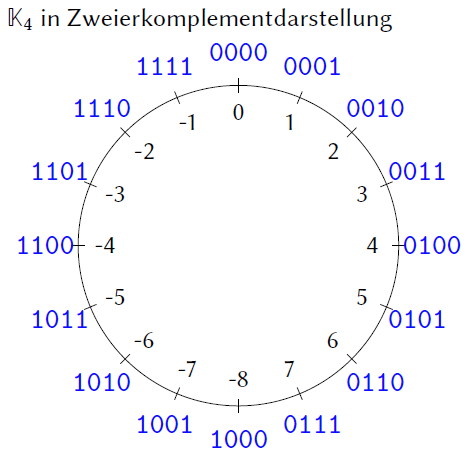
\includegraphics[scale=0.45]{ZK_K4}
	\end{figure}
	
\end{frame}

\begin{frame}{Zweierkomplement (ZK)}
	
	Ermöglicht Binärdarstellung positiver \textbf{und} negativer Zahlen. \\
	Besonders hardwareverträglich verglichen mit anderen Darstellungen \textit{(mehr dazu in Technischer Informatik)}.

	\begin{block}{Definition}
		Wollen Zweierkomplement der Länge $\ell$. \\ Haben $\fbin_\ell$: einfache Konvertierung nach Binär mit Länge $\ell$.
		$$\fZkpl_\ell(x) = \begin{cases} \word 0 \fbin_{\ell-1}(x), & \text{falls } x \geq 0 \\ 
										 \word 1 \fbin_{\ell-1}(2^{\ell-1}+x) & \text{falls } x < 0\end{cases}$$
		
		Äquivalent:
		$$\fZkpl_\ell(x) = \begin{cases} \fbin_{\ell}(x), & \text{falls } x \geq 0 \\ 
										 \fbin_{\ell}(2^{\ell}+x) & \text{falls } x < 0\end{cases}$$
	\end{block}
\end{frame}

\begin{frame}{ZK ausrechnen}
	$x \geq 0$: geschenkt \smiley \\
	$x < 0$:
	\begin{enumerate}
		\item Binärdarstellung von $\abs{x}$ berechnen
		\item Vorne mit Nullen auffüllen bis zur Länge $\ell$
		\item Alle binären Ziffern negieren
		\item 1 addieren
	\end{enumerate}
	
	\begin{Beispiel}
		 $$\fZkpl_4(-2): 2 \stackrel{\fRepr_2}{\?>} \word{10} \stackrel{\text{Nullen}}{\?>} \word{0010} \stackrel{\text{negieren}}{\?>} \word{1101} \stackrel{+1}{\?>} \underline{\word{1110}}. $$
		 Achtung, das ist \textbf{keine offizielle Schreibweise!} Das will ich auf'm Übungsblatt nicht sehen!
	\end{Beispiel}
\end{frame}

\begin{frame}{ZK ausrechnen}
	\begin{Beispiel}
		\begin{align*}
		\fZkpl_5(0)  &= \visible<2->{\word{00000}} \\
		\fZkpl_5(2) &= \visible<3->{\word{00010}} \\
		\fZkpl_5(15) &= \visible<4->{\word{01111}} \\
		\fZkpl_5(-1) &= \visible<5->{\word{11111}} \\
		\fZkpl_5(-6) &= \visible<6->{\word{11010}} \\
		\fZkpl_5(-16) &= \visible<7->{\word{10000}}
		\end{align*}
	\end{Beispiel}
\end{frame}

\begin{frame}{ZK ausrechnen -- formal}
	Die einzelnen Schritte können wir auch formal angeben:\\
	(Wir operieren jeweils auf Wörtern aus $\{\word 0, \word 1\}^* = Z_2^*$) \\[0.5em]
	1. Binärdarstellung von $\abs{x}$ berechnen: $Repr_2(\abs{x})$ \\
	2. Vorne mit Nullen auffüllen bis zur Länge $\ell$\\ \pause
	\begin{threealign}
		Fill_\ell : Z_2^m &\functionto& Z_2^\ell \qquad (m \le \ell) \\ \visible<3-> {
		w &\mapsto& \begin{cases}
		\word 0^\ell, & w = \varepsilon \\
		Fill_{\ell-1}(w') \cdot \mu, & w = w' \cdot \mu \text{ mit } w' \in Z_2^*, \mu \in Z_2
		\end{cases} \\
		\text{Oder viiieeel einfacher: }& \\
		w &\mapsto& \begin{cases}
		w, & \setsize{w} = \ell \\
		Fill_\ell(\word 0 w), & \text{sonst}
		\end{cases} \\
	}
	\end{threealign}
	\pause[4] 3. / 4. Analog %TODO
\end{frame}

\begin{frame}{Von einer Zahlendarstellung zur Anderen}
	\vspace{-.2\baselineskip}
	Von Basis $a$ nach Basis $b$ -- eigentlich recht intuitiv:
	$$\fTrans_{b,a} = \fRepr_b \after \fNum_a$$
	Z.~B.
	$$\fTrans_{3,5} = \fRepr_3 \after \fNum_5$$
\end{frame}
\begin{frame}{Von einer Zahlendarstellung zur Anderen}
	\begin{block}{Aufgabe}
		Berechne folgende Darstellungen:\\
		\begin{enumerate}[(1)]
			\item $\fRepr_2(42) = \visible<1->{ \word{101010}_2}$ 
			\item $\fTrans_{4,2}(\word{101010}) = \visible<2->{ \word{222}_4}$ 
			\item $\fTrans_{8,10}(\word{42}) = \visible<3->{ \word{52}_8}$ 
			\item $\fTrans_{16,10}(\word{42}) = \visible<4->{ \word{2A}_{16}}$
		\end{enumerate}
	\end{block}

	Was ist bei allen Wörtern gleich? \only<5->{\impl Die Bedeutung!} \\
	Was macht die Rechnungen (2) -- (4) vergleichsweise einfach? \pause[6] \\
	\impl Wir können die Struktur ausnutzen und zeichenweise vorgehen! ($\fTrans_{8,10}(\word{42}) = \fTrans_{8,2}(\word{101} \cdot \word{010}) = \fTrans_{8,2}(\word{101}) \cdot \fTrans_{8,2}(\word{010})$)
\end{frame}

\section{Codierungen}

\begin{frame}{Übersetzungen}
	\textbf{Übersetzung:} „Bedeutungserhaltende“ Abbildung \\[0.5em] \pause
	\textbf{Codierung:} Injektive Übersetzung \\ \pause
	\begin{itemize}
		\item Injektiv reicht, weil wir jedem $f(w)$ sein erzeugendes $w$ zuordnen können
		\implitem Definiere Bedeutung von $f(w) := \text{Bedeutung von } w$
	\end{itemize}
	
	\pause
	\begin{itemize}
		\item \textbf{Problem}: \emph{Beliebige} Codierungen zu speichern sehr aufwendig
		\item Wenn $\abs{\text{Definitionsbereich}} = \infty$ \impl sogar unmöglich!
		\implitem Bringen wir etwas Struktur ins Spiel!
	\end{itemize}
\end{frame}

\begin{frame}{Homomorphismen}
	Ein \textbf{Homomorphismus} ist eine \textit{strukturerhaltende} Abbildung \\ \pause
	\begin{threealign}
		\Phi : A &\functionto& B \\
		\text{ mit } \forall x,y \in A: \quad  \Phi(x \sim y) &=& \Phi(x) \bowtie \Phi(y)
	\end{threealign}
	\medskip \\
	Dabei stehen $\sim$ und $\bowtie$ hier für feste beliebige Operationen, wie z.~B. $+, -, \*, /, \oplus, \barwedge, ...$ \\
	(Muss es auf $A$ bzw. $B$ natürlich geben!)
\end{frame}

\begin{frame}{Homomorphismen}
	In GBI: Homomorphismen auf Wörtern mit „$\*$“ als Operation.\\
	\impl $A, B$ Alphabete, dann ist $h: A^* \functionto B^*$ ein Homomorphismus, wenn
	$$ \forall x, y \in A^* : \quad h(x \cdot y) = h(x) \cdot h(y). $$
	
	\pause
	\impl Brauchen nur Funktionswerte für einzelne Zeichen $a \in A$, dann kennen wir schon das ganze $h$! \\
	\impl Brauchen uns nur eine Tabelle für die Zeichen zu merken \\
	\impl $A$ endlich \impl Tabelle endlich \impl gut speicherbar
	
	\pause
	\begin{Beispiel}
		Sei $h$ ein Homomorphismus, für den gilt: $h(\word a) = \word 2, h(\word b) = \word 3$. \\
		Dann gilt $h(\word{aba}) = h(\word a) \cdot h(\word b) \cdot h(\word a) = \word{232}. $ \\[0.5em]
		\pause
		$\fTrans_{2,16}$ ist fast ein Homomorphismus (führende Nullen machen Probleme)\\
		$\fTrans_{3,2}$ ist kein Homomorphismus (siehe dazu ÜB WS15/16)
	\end{Beispiel}
\end{frame}

\begin{frame}{Homomorphismen bauen}
	Haben: Abbildung der einzelnen Zeichen \\
	Wollen: Abbildung ganzer Wörter 
	\begin{Definition}
		Sei $f: A \functionto B^*,$ \pause definiere $f^{**}:A^* \functionto B^*$ als
		\begin{align*}
		f^{**}(\eps) &= \eps  \\
		\forall w\in A^*, x\in A: \quad  f^{**}(w \* x) &= f^{**}(w) \* f(x)       
		\end{align*}
	\end{Definition}

	$f^{**}$ heißt der durch $f$ \textbf{induzierte} Homomorphismus.
\end{frame}

\begin{frame}{$\eps$-Freiheit}
	Klar ist: Für jeden Hom. $h$ ist $h(\eps) = \eps$.
	
	\pause
	\begin{Definition}
		Ein Homomorphismus heißt $\eps$-frei, wenn 	$$ \forall x\in A : h(x) \neq \eps. $$
	\end{Definition}

	
	Was ist das Problem mit Homomorphismen, die nicht $\eps$-frei sind? \\ \pause
	\impl Es geht Information verloren.\\
	
	\begin{Beispiel}
		Sei $h$ ein Hom. mit $h(\word c) = \eps, \; h(\word b) = \word 2$. \\
		Haben unbekanntes $w \in \{\word b, \word c\}^*$ und wissen: $h(w) = \word 2$. \\
		\smallskip
		Wie kommen wir von $h(w)$ wieder zu $w$ zurück? \\ \pause
		\impl Gar nicht! (Wissen nicht, wieviel \word c in $w$ drin sind.)
	\end{Beispiel}
\end{frame}

\begin{frame}{Präfixfreiheit}
	\begin{Definition}
		Ein Homomorphismus heißt \textbf{präfixfrei}, wenn für
		\emph{keine} zwei verschiedenen Symbole $x_1,x_2\in A$ gilt: $h(x_1)$
		ist ein Präfix von $h(x_2)$.
	\end{Definition}

	\bigskip
	Was ist das Problem mit Homomorphismen, die nicht präfixfrei sind? \\ \pause
	\impl Es geht Information verloren.\\
	
	\begin{Beispiel}
		Sei $h$ ein Hom. mit $h(\word a) = \word 2, \; h(\word b) = \word 3, \; h(\word c) = \word{23}$. \\ 
		Haben unbek. $w \in \{\word a, \word b, \word c\}^*$ und wissen: $h(w) = \word{23}$. \\
		\smallskip
		Wie kommen wir von $h(w)$ wieder zu $w$ zurück?\\ \pause
		\impl Gar nicht! $w = \word c$ oder $w = \word{ab}$, wir wissen es nicht!
	\end{Beispiel}
	
\end{frame}

\begin{frame}{Zurück zu Codierungen}
	\begin{block}{Beobachtung}
		Präfixfreie Homomorphismen sind $\eps$-frei.
	\end{block}

	\pause
	\begin{block}{Lemma}
		Präfixfreie Homomorphismen sind Codierungen (also injektiv).
	\end{block}

	\pause
	\begin{block}{Beobachtung}
		Präfixfreie Codes kann man \enquote{einfach} decodieren:
		\[
		u(w) = 
		\begin{cases}
		\eps, & \text{ falls } w=\eps\\
		x\*u(w'), & \text{ falls } w=h(x) \* w' \text{ für ein } x\in A \\
		\bot,  & \text{ sonst }\\
		\end{cases}
		\]
	\end{block}
	% ($\bot$: „undefiniert“, „bottom“.)
	
\end{frame}

\begin{frame}{Decodierung: Übung}
	Erinnerung – Decodierungsfunktion:
	\[
	u(w) = 
	\begin{cases}
	\eps, & \text{ falls } w=\eps\\
	x\*u(w'), & \text{ falls } w=h(x) \* w' \text{ für ein } x\in A \\
	\bot,  & \text{ sonst }\\
	\end{cases}
	\]
	\begin{block}{Aufgabe}
	Decodiert das folgende Codewort mit der jeweiligen Codierung:\\
	\word{011000000001}
	\smallskip
	
	(1) $f(\word E) = \word{10} \quad f(\word M) = \word{01} \quad f(\word A) = \word{0001} \quad f(\word T) = \word{0000}$ \\
	\visible<2->{\word{META}} 
	\smallskip
	(2) $f(\word E) = \word 1 \quad f(\word M) = \word 0 \quad f(\word A) = \word{0001} \quad f(\word T) = \word{0000}$ \\
	\visible<3->{Nicht eindeutig möglich, da nicht präfixfrei.}
	\end{block}
\end{frame}

\section{Huffman-Codierung}

\begin{frame}
	Kann eine Codierung auch helfen, Zeichen zu sparen? \\
	\pause
	\impl Klar: \textbf{Komprimierung}!
\end{frame}

% too little time...
\only<beamer:0>{\xkcdframe{1683}{Digital Data}{2.5}}

\begin{frame}{Huffman-Codierungen}
	\begin{block}{Was ist das?}
		Eine \textbf{Huffman-Codierung} ist...
		\begin{itemize}
			\item ein präfixfreier Homomorphismus {\small (\impl einfach zu decodieren)}, sodass...
			\item Codierung eines Zeichens umso länger, je seltener das Zeichen vorkommt
		\end{itemize}
	\end{block}
	
	Die Huffman-Codierung für ein Wort ist dabei \textit{nicht eindeutig} (sehen wir gleich).
	\pause
	\begin{block}{Lemma}
		Unter allen präfixfreien Codes führen Huffman-Codes zu kürzesten Codierungen
		\textbf{des Wortes, für das die Huffman-Codierung konstruiert wurde.}
	\end{block}
\end{frame}

\begin{frame}{Konstruktionsverfahren}
	Kochrezept für einen Huffman-Baum zu einem geg. Wort:
	\begin{enumerate}
		\item Für jedes Zeichen die \emph{Häufigkeit} ermitteln
		\item Alle Zeichen mit ihrer Häufigkeit als \emph{Blätter} in die unterste Ebene zeichnen
		\item Nehme die zwei Knoten {\small (nicht unbedingt Blätter!)} mit \emph{geringsten Häufigkeiten} und lege einen Parent darüber an mit der Summe ihrer Häufigkeiten
		%\item Jeweils die zwei Knoten (nicht unbedingt Blätter!) mit den geringsten Häufigkeiten \enquote{verbinden}(also einen neuen Knoten darüber anlegen, der die Summe der Häufigkeiten erhält)
		\item Wiederhole (3), bis der ganze Baum aufgebaut ist.
		\item Die linken Äste mit \word 0 beschriften, die rechten Äste mit \word 1.
		\item Codierungen der Zeichen ablesen
		\item Ausgangswort codieren (wenn gefordert, nicht vergessen!)
	\end{enumerate}
\end{frame}

\begin{frame}{Beispiel}
	Gegeben: $w= \word{abadcadaac} $ (10 Zeichen) \\[1em]
	
	\only<1-3|handout:1>{ \visible<3>{
	\begin{minipage}{0.6\linewidth}
		\begin{figure}[b]
			\centering
			\begin{tikzpicture}
			[level 1/.style={sibling distance=40mm},
			level 2/.style={sibling distance=20mm},
			level 3/.style={sibling distance=15mm}]
			\node {$10$}
			child {
				node{$5$}
				child{
					node{$3$}
					child{
						node{$1,\word b$}
						edge from parent node[left] {\word 0}
					}
					child {
						node{$2,\word d$}
						edge from parent node[right] {\word 1}
					}
					edge from parent node[left] {\word 0};
				}
				child{
					node{$2,\word c$}
					edge from parent node[right] {\word 1}
				}
				edge from parent node[left] {\word 0\ \mbox{}};
			}
			child{
				node{$5,\word a$}
				edge from parent node[right] {\ \word 1}
			};
			\end{tikzpicture}
		\end{figure}  
	\end{minipage}
	}}
	\only<4-|handout:2> {
		\begin{minipage}{0.6\linewidth}
			Wie lang wird das codierte Wort $h(w)$?\\ \visible<5->{ 
			$5\*1 + 1\*3 + 2\*2 + 2\*3 = 18$ Zeichen\\ 
			Ähm, mehr Zeichen als vorher!? WTF? \\
			\visible<6->{\impl Keine Panik: \\
				Um ein Zeichen aus $\word a, \word b, \word c, \word d$ zu codieren, brauchen wir mindestens 2~Bit {\small (da 4 Möglichkeiten)}. \\ 
				Für die Zeichen $\word 0, \word  1$ brauchen wir aber nur ein Bit.  \\
				\impl 18 Bit statt 20 Bit \impl Platz gespart. \smiley
		}}
		\end{minipage}
	}
	\visible<2-> {
		\begin{minipage}{0.2\linewidth}
			\hfill
			\hfill 
			\vspace*{0.1\linewidth}
			\begin{table}[H]
				\begin{tabular}{c|cccc}
					\hline
					$x$ & \word a & \word b & \word c & \word d  \\ \hline
					$|w|_x$  & 5 & 1 & 2 & 2 \\ \hline
					$h(x)$ & \visible<3->{\word 1 & \word{000} & \word{01} & \word{001}} \\ \hline 
				\end{tabular}
			\end{table}
		\end{minipage}
	}
\end{frame}

\begin{frame}{Huffman-Codes}
		Huffman-Codierungen funktionieren immer nur gut für Wörter, die eine \textbf{ähnliche relative Zeichenhäufigkeit} haben wie das Wort, für das der Code erstellt wurde.
  \end{frame}
%   \begin{frame}{Huffman-Codes}
% 		\begin{Beispiel}
% 			$w_1 = \word{badcfehg}, \quad w_2 = \word a^1 \word b^2 \word c^4 \word d^8 \word e^{16} \word f^{32} \word g^{64} \word h^{128}$. \\
% 			Erstellt eine Huffman-Codierung für jedes Wort und codiert $w_1$ mit beiden Codierungen.\\
% 			Was verhalten sich die Längen der Codewörter?
% 			\visible<2->{
% 				\newcommand{\css}{\;\,}
% 				%\vspace{-.8\baselineskip}
% 				\begin{columns}[T] 
% 					\begin{column}[T]{.65\textwidth} 
% 							\begin{tabular}{c|c@{\css}c@{\css}c@{\css}c@{\css}c@{\css}c@{\css}c@{\css}c}
% 								\hline
% 								$x$ & \word a & \word b & \word c & \word d & \word e & \word f & \word g & \word h \\ \hline
% 								$|w_1|_x$  & 1 & 1 & 1 & 1 & 1 & 1 & 1 & 1 \\ \hline
% 								$h_1(x)$ & \word{000} & \word{001} & \word{010} & \word{011} & \word{100} & \word{101} & \word{110} & \word{111} \\ \hline 
% 							\end{tabular}
% 							\forcenewline\vspace{.3\baselineskip}
% 							\begin{tabular}{c|c@{\css}c@{\css}c@{\css}c@{\css}c@{\css}c@{\css}c@{\css}c}
% 								\hline
% 								$x$ & \word a & \word b & \word c & \word d & \word e & \word f & \word g & \word h \\ \hline
% 								$|w_2|_x$  & 1 & 2 & 4 & 8 & 16 & 32 & 64 & 128 \\ \hline
% 								$h_2(x)$ & $\word{1}^7$ & $\word{1}^6\word{0}$ & $\word{1}^5\word{0}$ & $\word{1}^4\word{0}$ & $\word{1}^3\word{0}$ & \word{110} & \word{10} & \word 0 \\ \hline 
% 							\end{tabular}
% 					\end{column}
% 					\hspace{-2\baselineskip}
% 					\begin{column}[T]{.35\textwidth} 
% 						\bigskip
% 						$\size{h_1(w_1)} = 8 \* 3 = 24$ \\
% 						$\size{h_1(w_2)} = 255 \* 3 = 765$ \\
% 						\bigskip
% 						\bigskip
% 						$\size{h_2(w_1)} = 35$ \\
% 						$\size{h_2(w_2)} = 501$
% 					\end{column}
% 				\end{columns}
				
% 			}
% 		\end{Beispiel}
% \end{frame}


\begin{frame}{Huffman-Codes}
	\begin{block}{Erweiterung}
		Wir können nicht nur einzelne Buchstaben codieren. \\
		Bei $ w = \word a^{10} \word b^{10} \word c^{10} $ lohnt es sich, pro Block gleicher Buchstaben eine Codierung zu haben.
	\end{block}
\end{frame}


\subsection{Aufgaben}
\begin{frame}{Aufgabe (WS 2008) }
	Das Wort $$w = \word{0000\only<3->{\text{ }}0001\only<3->{\text{ }}0011\only<3->{\text{ }}0001\only<3->{\text{ }}0011\only<3->{\text{ }}0000\only<3->{\text{ }}0000\only<3->{\text{ }}1110\only<3->{\text{ }}0001\only<3->{\text{ }}0000}$$ soll komprimiert werden.
	
	\pause
	\begin{itemize}[<+->]
		\item[a)] Zerlegen Sie $w$ in Viererblöcke und bestimmen Sie die Häufigkeiten der vorkommenden Blöcke.
		\item[b)] Zur Kompression soll ein Huffman-Code verwendet werden. Benutzen Sie die in Teilaufgabe a) bestimmten Häufigkeiten, um den entsprechenden Baum aufzustellen. Beschriften Sie alle Knoten und Kanten.
		\item[c)] Geben Sie die Codierung des Wortes $w$ mit Ihrem Code an.
	\end{itemize}
\end{frame}

\begin{frame}{Lösung}
	$$w = \word{0000000100110001001100000000111000010000}$$
	\textit{a) Zerlegen Sie $w$ in Viererblöcke und bestimmen Sie die Häufigkeiten der vorkommenden Blöcke.} \\[1em]
	\pause
	$$w = \word{0000 0001 0011 0001 0011 0000 0000 1110 0001 0000}$$ \pause
	\begin{table}[h!]
		\centering
		\begin{tabular}{l|cccc}	
			& \word{0000} & \word{0001} & \word{0011} & \word{1110} \\ \hline
			Absolute Häufigkeiten: & 4 & 3 & 2 & 1 \\
			Relative Häufigkeiten:  & 0.4 & 0.3 & 0.2 & 0.1\\
		\end{tabular}
	\end{table}
\end{frame}

\begin{frame}{Lösung}
	\textit{b) Zur Kompression soll ein Huffman"=Code verwendet werden. Benutzen Sie die in Teilaufgabe a) bestimmten Häufigkeiten, um den entsprechenden Baum aufzustellen. Beschriften Sie alle Knoten und Kanten.}
	\begin{minipage}{0.45\linewidth}
		
		\pause 
		\begin{table}[h!]
			\centering
			\begin{tabular}{cccc}	
				\word{0000} & \word{0001} & \word{0011} & \word{1110} \\ \hline
				4 & 3 & 2 & 1 \\	
			\end{tabular}
		\end{table}
	\end{minipage}
	\hfill
	\begin{minipage}{0.5\linewidth}
		\begin{figure}[h!]
			\centering
			\visible<3>{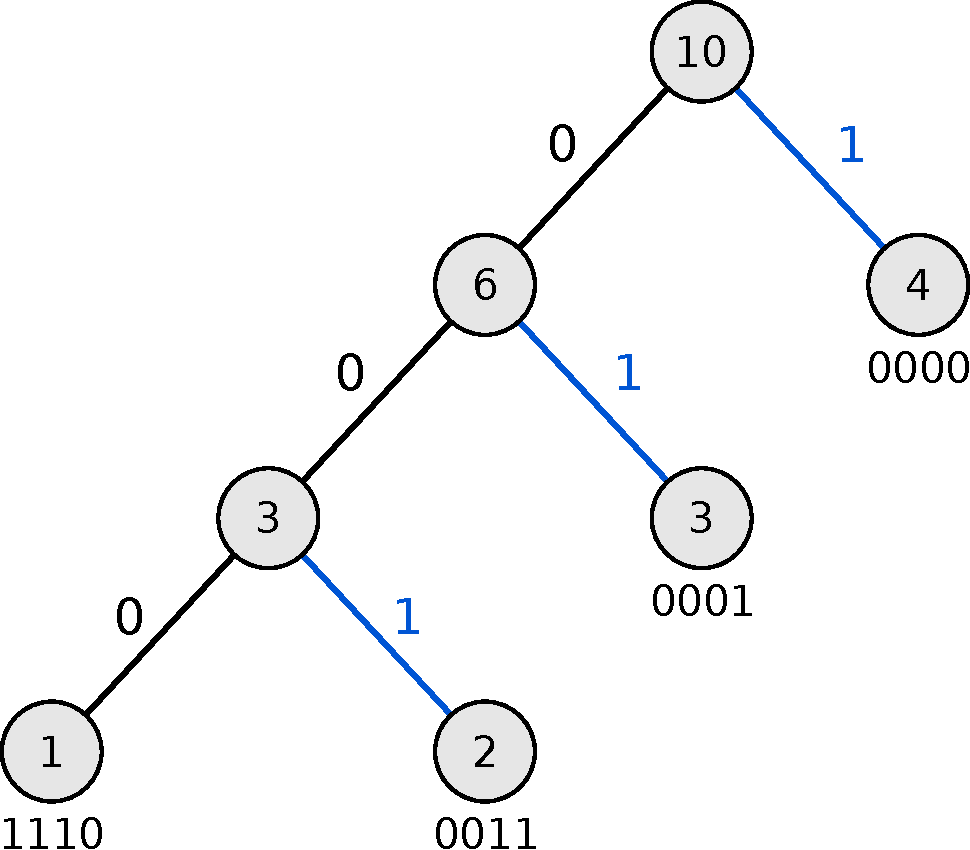
\includegraphics[scale=0.35]{Huffman.pdf}}
		\end{figure}
	\end{minipage}
\end{frame}

\begin{frame}{Lösung}
	\textit{c) Geben Sie die Codierung des Wortes $w$ mit Ihrem Code an.} \\[2em] \pause
	\begin{align*}
		h(&\word{0000000100110001001100000000111000010000}) = \\
		  &\word{1010010100111000011}
	\end{align*}
\end{frame}

%\begin{frame}
%	\frametitle{Aufgabe (WS 2010)}
%	Seien $n, k \in \N_0$ mit $1 \leq k \leq n$. In einem Wort $w \in \{a, b, c\}^\ast$ der Länge $3n$ komme $k$ mal das Zeichen $a$, $n$ mal das Zeichen $b$ und $2n - k$ mal das Zeichen $c$ vor.
%	\begin{itemize}
%		\item Geben Sie den für die Huffman-Codierung benötigten Baum an.
%		\item Geben Sie (in Abhängigkeit von $k$ und $n$) die Länge des zu $w$ gehörenden Huffman-Codes an.
%	\end{itemize}
%\end{frame}
%
%\begin{frame}
%	\frametitle{Lösung}
%	\vspace*{1em}
%	\begin{minipage}{0.45\linewidth}
%		\textit{$\dots$ Länge $3n$ komme $k$ mal das Zeichen $a$, $n$ mal das Zeichen $b$ und $2n - k$ mal das Zeichen $c$ vor. \\[1em] Geben Sie den für die Huffman-Codierung benötigten Baum an.} 
%		\pause
%		\begin{table}[h!]
%			\centering
%			\begin{tabular}{ccc}	
%				$a$ & $b$ & $c$ \\ \hline
%				$k$ & $n$ & $2n-k$ \\	
%			\end{tabular}
%		\end{table}
%		\pause
%		$$k \leq n \leq 2n -k $$ $$ n+k+2n-k = 3n$$
%	\end{minipage}
%	\hfill
%	\begin{minipage}{0.5\linewidth}
%		\begin{figure}[h!]
%			\centering
%			\only<4>{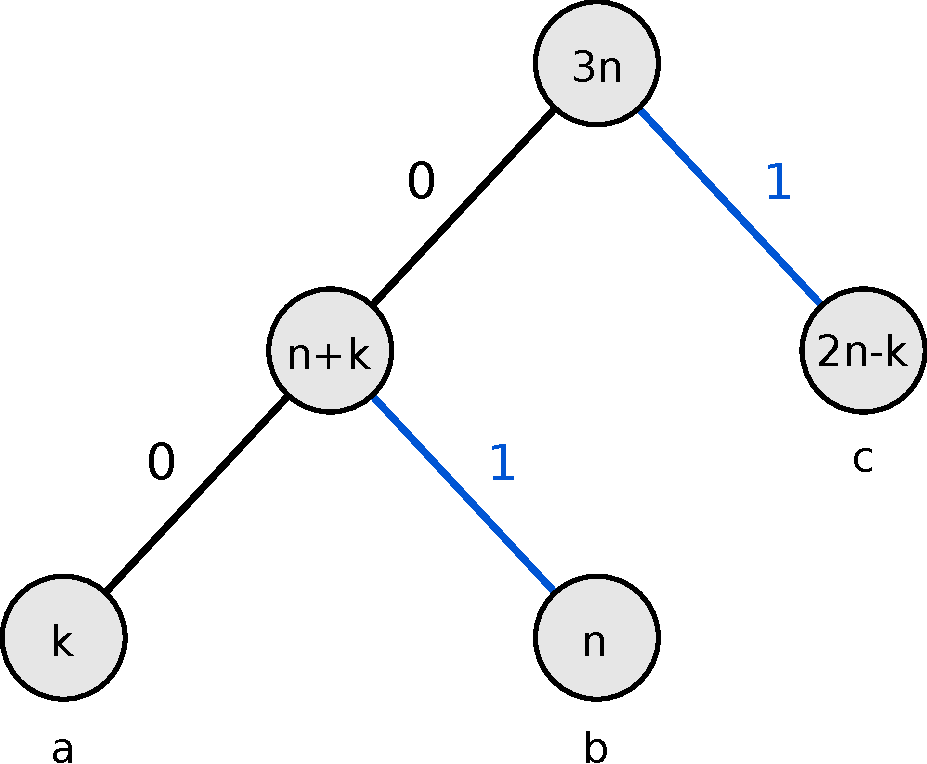
\includegraphics[scale=0.35]{Huffman2.pdf}}
%		\end{figure}
%	\end{minipage}
%\end{frame}
%
%\begin{frame}
%	\frametitle{Lösung}
%	\textit{Geben Sie die Länge des zu $w$ gehörenden Huffman-Codes an.} \\[2em]
%	\pause
%	Jedes $a$ und jedes $b$ wird durch zwei Zeichen codiert, und jedes $c$ wird durch ein Zeichen codiert. Damit erhält man insgesamt $$2k + 2n + 2n - k = 4n + k$$ Zeichen in der Codierung.
%\end{frame}


\begin{frame}{Ausblick}
	Die Huffman-Codierung hat ein Problem: Zum Decodieren muss der Huffman-Baum bekannt sein. Möglichkeiten:
	\begin{enumerate}
		\item Der Codebaum wird vor dem eigentlichen Codewort angegeben.\\ 
		\emph{Problem}: Das verlängert das Codewort.
		\item Es wird ein vorher festgelegter Codebaum verwendet.\\
		 \emph{Problem}: Dieser Codebaum kann evtl. sehr schlechte Ergebnisse liefern, da nicht für alle Wörter geeignet
	\end{enumerate}

	Diese Probleme können durch andere Codierungsverfahren gelöst werden, indem z.B. das Wörterbuch dynamisch während der Decodierung aus dem Codewort aufgebaut wird (z.~B. Lempel-Ziv-Welch-Verfahren).
\end{frame}



\appendix
\beginbackup

\section{Zusammenfassung und Ausblick}

\begin{frame}	
	\begin{block}{Was ihr nun wissen solltet}
		\begin{itemize}
			\item Wie man Zahlen anders darstellt
			\item Wie man das Zweierkomplement bildet
			\item Übersetzungen und Codierungen
			\item Huffman-Codierung
		\end{itemize}
	\end{block}
	
	\begin{block}{Was nächstes Mal kommt}
		\begin{itemize}
			\item Speicher -- Damit wir nicht alles gleich wieder vergessen
			\item MIMA -- Den Bits beim Arbeiten zuschauen
		\end{itemize}
	\end{block}
\end{frame}



\only<handout:0>{\slideThanks}

\xkcdframe{571}{Danke für eure Aufmerksamkeit! \smiley}{2.5} % Zweierkomplement
% \lastframe{0.75}{0}{xkcd/tar.png}{https://www.xkcd.com/1168/} % Komprimierung

\only<beamer:0>{\slideThanks}

\backupend

\end{document}